\documentclass[12pt]{article}
\usepackage[a4paper,margin=0.75in]{geometry}
\usepackage[utf8]{inputenc}
\usepackage[OT1]{fontenc}
\usepackage[table,usenames,dvipsnames]{xcolor}
\usepackage{array}
\usepackage{varwidth}
\usepackage{tabularx}
\usepackage{amsmath}
\usepackage{hyperref}
\usepackage{enumitem}
\usepackage{graphicx}
\usepackage{tcolorbox}
\renewcommand*\familydefault{\sfdefault}

\newtcolorbox{mybox}[3][]
{
  colframe = #2!25,
  colback  = #2!10,
  coltitle = #2!20!black,  
  title    = {#3},
  #1,
}

\hypersetup{
    colorlinks=true,
    linkcolor=blue,
    filecolor=magenta,      
    urlcolor=cyan,
    pdftitle={Overleaf Example},
    pdfpagemode=FullScreen,
}

\title{\textbf{COL774 Assignment 2}}
\author{Aniruddha Deb \\ \texttt{2020CS10869}}
\date{October 2022}

\begin{document}

\maketitle

\section{Naive Bayes}

\begin{enumerate}[label=(\alph*)]
  
    \item Naive Bayes was implemented using the \textbf{Multinomial Event Model} as discussed in class, which uses the frequency of the words rather than just their presence. The vocabulary was learnt from the training dataset, and any words not in the vocabulary in the test dataset were ignored. With this implementation, the following results were obtained:
    \begin{enumerate}[label=\roman*.]
        \item An accuracy of $79.313\%$ on the test dataset, with 7501/10000 positive examples and 4396/5000 negative examples correctly classified
        \item The following word clouds were obtained. Note that there are a lot of stopwords, which we remove in part (d)
    \end{enumerate}
    \begin{center}
        \begin{tabular}{c c}
            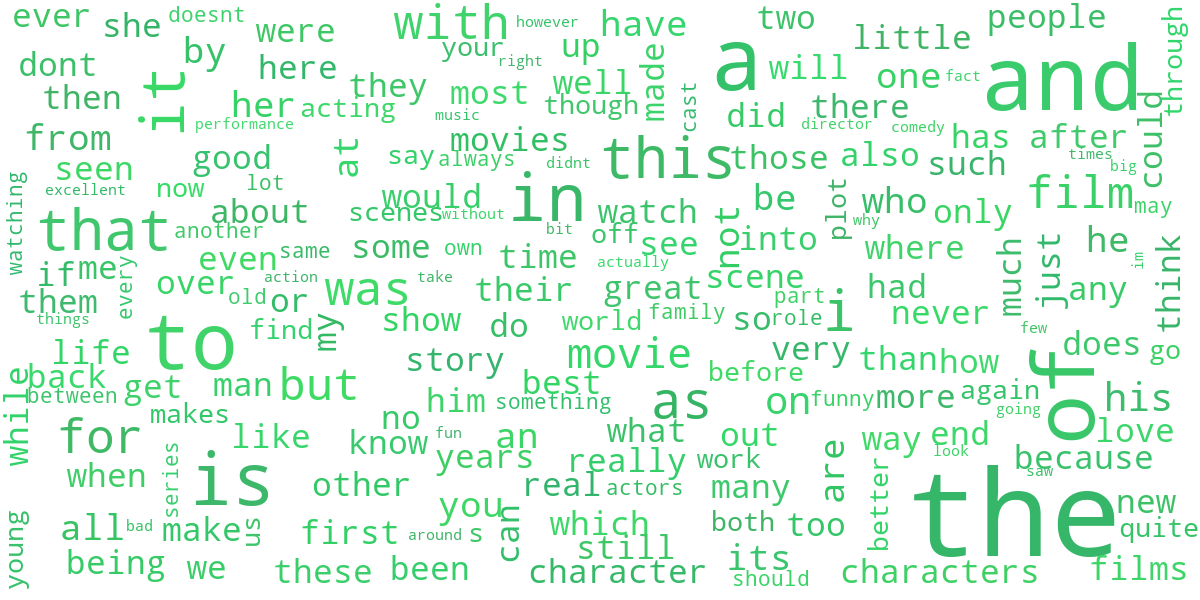
\includegraphics[width=0.44\textwidth]{../Q1/Qa/wc_pos.png} & 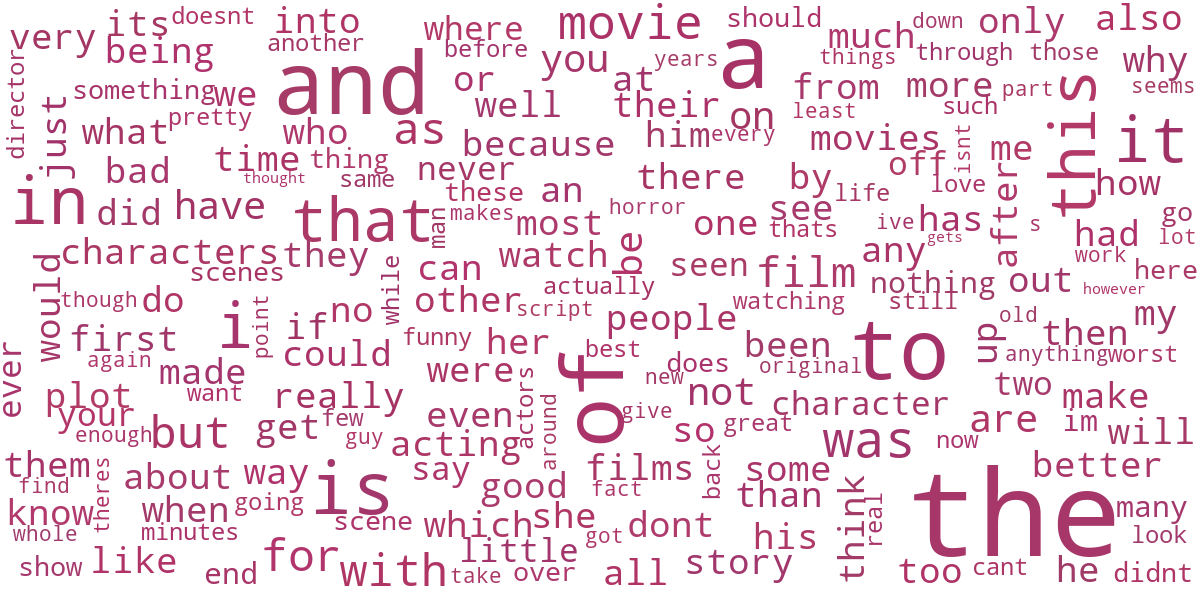
\includegraphics[width=0.44\textwidth]{../Q1/Qa/wc_neg.png} \\
            Positive reviews & Negative reviews
        \end{tabular}
    \end{center}
    
    \item With Random Guessing, we'd obtain a test set accuracy of approximately 50\%. By simply predicting each sample as positive, this would jump to 66.6\%, as the number of positive reviews in the test set is twice the number of negative reviews.

    Our Algorithm gives a 30\% increase in accuracy over random guessing and a 14\% increase in accuracy over simply predicting each review as positive.

    \item The confusion matrices are as follows:

    \begin{center}
    \begin{tabular}{c c c}
        NaiveBayes & Random & AllPositive \\
        \begin{tabular}{r|c|c|}
            & AP & AN \\
            \hline
            PP & 7501 & 604 \\
            \hline
            PN & 2499 & 4396 \\
            \hline
        \end{tabular} & 
        \begin{tabular}{r|c|c|}
            & AP & AN \\
            \hline
            PP & 5000 & 2500 \\
            \hline
            PN & 5000 & 2500 \\
            \hline
        \end{tabular} &
        \begin{tabular}{r|c|c|}
            & AP & AN \\
            \hline
            PP & 10000 & 5000 \\
            \hline
            PN & 0 & 0 \\
            \hline
        \end{tabular} 
    \end{tabular}
    \end{center}

    The highest sum of diagonal entries is in the Naive Bayes classifier. This implies that the accuracy (number of correctly classified samples) of Naive Bayes is better than randomly or selectively guessing.

    The pattern is that the column sums for the actuals always add up to the number of examples of that category in the training set. This is because the actual column measures the number of actual examples in the dataset, and across all predictions, would sum to the total number of that category in the dataset.

    \item Removing stopwords and stemming gives us an accuracy of \textbf{80.4\%}, with 7678/10000 positive reviews and 4388/5000 negative reviews correctly classified.

    \begin{center}
        \begin{tabular}{c c}
            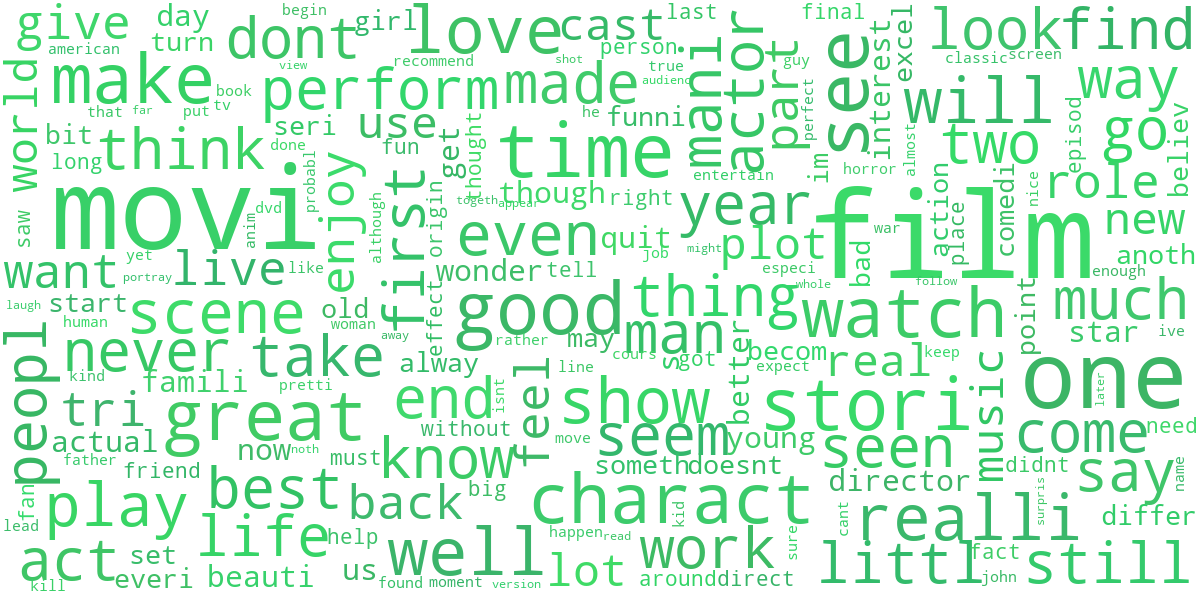
\includegraphics[width=0.44\textwidth]{../Q1/Qd/wc_pos.png} & 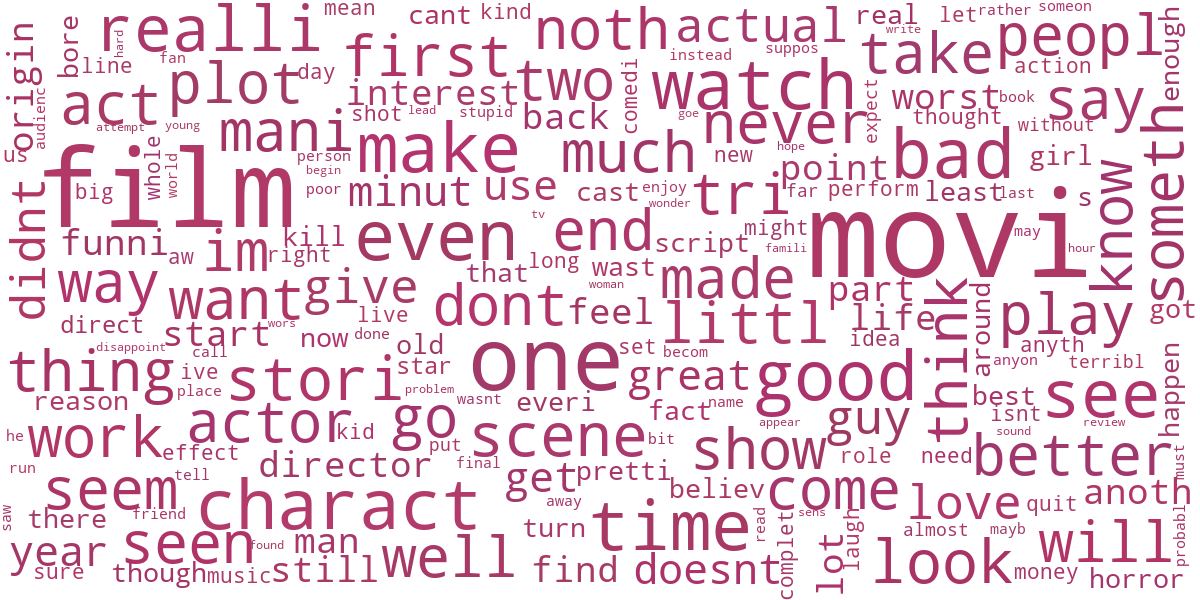
\includegraphics[width=0.44\textwidth]{../Q1/Qd/wc_neg.png} \\
            Positive reviews & Negative reviews
        \end{tabular}
    \end{center}

    The word clouds show the frequency of the various word stems rather than the frequency of the words themselves.

\item Using Bigrams (in addition to removing stopwords and stemming) gives us an accuracy of \textbf{84.4 \%}, with 8209/10000 positive reviews and 4447/5000 negative reviews correctly classified.

    For the additional feature, we use Trigrams. Using trigrams, in addition to bigrams and removing stopwords + stemming gives us an accuracy of \textbf{85.2 \%}, with 8352/10000 positive reviews and 4423/5000 negative reviews correctly classified.

    The additional sets of features do help us improve our accuracy (explain why)

\item The best-performing (most accurate) model is the Trigram model, which has a precision of 8352/(8352+577) = 0.935, a recall of 8352/(8352+1648) = 0.835 and an F1 score of $2(0.935 \times 0.835)/(0.935+0.835) = 0.882$

    The F1 score is a better metric for this dataset, as there are twice as many positive movie reviews in the test dataset compared to negative reviews. In this case, we can see significant accuracy gains by simply declaring everything as positive instead of proceeding class by class. The F1 score helps to prevent this from happening, and gives a more realistic representation of how accurate our model is, across both classes irrespective of how many samples there are in each class.

\end{enumerate}

\clearpage

\section{Binary SVM}

\begin{enumerate}[label=(\alph*)]
    \item \begin{enumerate}[label=\roman*.]
        \item With a threshold of $\alpha_i > 10^{-6}$ for the support vectors, we obtain \textbf{1528} support vectors, which is \textbf{38.2 \%} of the training set
        \item The test set accuracy we obtain is \textbf{79 \%} (1580/2000 test images were classified correctly)
        \item The top 5 support vectors are:

        \begin{center}
        \begin{tabular}{c c c c c}
            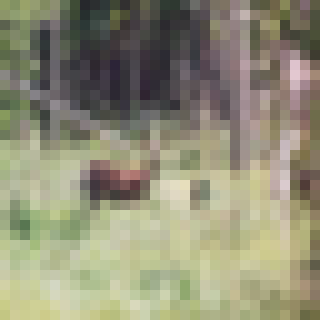
\includegraphics[width=0.1\textwidth]{../Q2/Qa/sv_1.png} &
            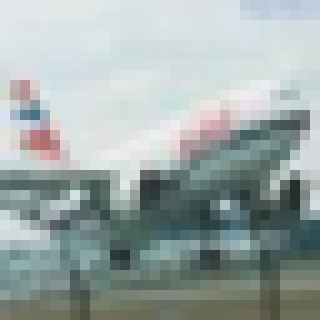
\includegraphics[width=0.1\textwidth]{../Q2/Qa/sv_2.png} &
            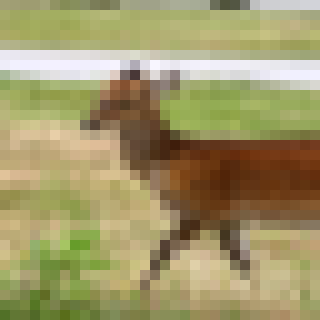
\includegraphics[width=0.1\textwidth]{../Q2/Qa/sv_3.png} &
            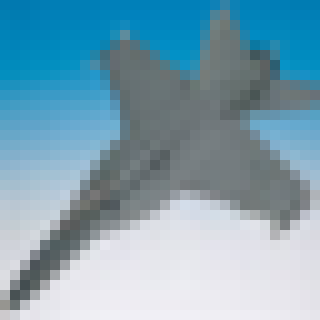
\includegraphics[width=0.1\textwidth]{../Q2/Qa/sv_4.png} &
            
\includegraphics[width=0.1\textwidth]{../Q2/Qa/sv_5.png} 
        \end{tabular}
        \end{center}

        The weight image is:

        \begin{center}
            
\includegraphics[width=0.1\textwidth]{../Q2/Qa/w.png} 
        \end{center}
    \end{enumerate}

    \item \begin{enumerate}[label=\roman*.]
        \item With a threshold of $\alpha_i > 10^{-6}$ for the support vectors and the given parameters, we obtain \textbf{1769} support vectors, which is \textbf{44.2 \%} of the training set. Out of these, \textbf{1143} support vectors overlap with the linear ones
        \item The test set accuracy we obtain is \textbf{85.75 \%} (1715/2000 test images were classified correctly)
        \item The top 5 support vectors are:

        \begin{center}
        \begin{tabular}{c c c c c}
            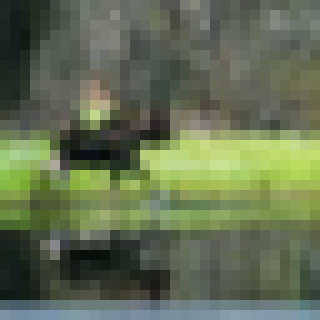
\includegraphics[width=0.1\textwidth]{../Q2/Qb/sv_1.png} &
            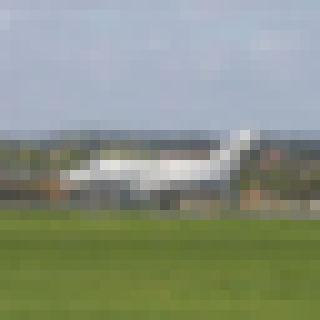
\includegraphics[width=0.1\textwidth]{../Q2/Qb/sv_2.png} &
            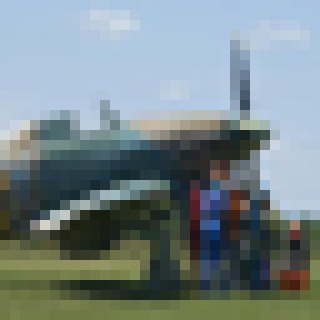
\includegraphics[width=0.1\textwidth]{../Q2/Qb/sv_3.png} &
            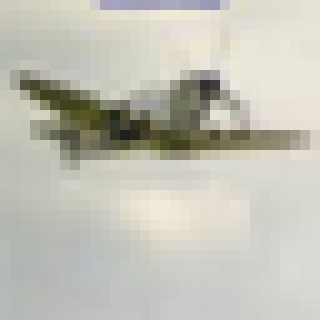
\includegraphics[width=0.1\textwidth]{../Q2/Qb/sv_4.png} &
            
\includegraphics[width=0.1\textwidth]{../Q2/Qb/sv_5.png} 
        \end{tabular}
        \end{center}

        \item The Gaussian Kernel allows for more fine-grained boundaries to be drawn between the datapoints, which 'fit' the shape of the data boundaries better compared to a linear separator. This is why the accuracy of the gaussian kernel is better than the linear kernel.
    \end{enumerate}

    \item \begin{enumerate}[label=\roman*.]
        \item For the Scikit-learn implementation, we obtain \textbf{1811} support vectors with a gaussian kernel and \textbf{1494} support vectors with a linear kernel. The pairwise overlaps are given below:
        \begin{center}
            \begin{tabular}{c c}
                & QP \\
                Scikit & 
            \begin{tabular}{c|c|c|}
                    & lin  & rbf  \\   
                \hline
                lin & 1494 & 1123 \\
                \hline
                rbf & 1130 & 1560 \\
                \hline
            \end{tabular}
            \end{tabular}
        \end{center}

    \item The normed difference of weights is $||w_{sk} - w_{qp}|| = 1571.61$, and the difference of biases is $b_{sk} - b_{qp} = -1.58$. Note that $b_{sk} = 0$.

    \item The test set accuracy we obtain is \textbf{86.95 \%} (1739/2000) for the RBF kernel and \textbf{79.1 \%} (1582/2000) for the linear kernel

        \item The training times are given below:
            \begin{center}
                \begin{tabular}{|l|c|}
                    \hline
                    Scikit RBF & 13.8 s \\
                    Scikit linear & 26.4 s\\
                    QP RBF & 58.1 s\\
                    QP linear & 47.7 s\\
                    \hline
                \end{tabular}
            \end{center}
    \end{enumerate}

\end{enumerate}

\section{Multiclass SVM}

\begin{enumerate}[label=(\alph*)]
    \item Using a multi-class variation of the CVXOPT solver with the same parameters as before ($\gamma = 0.001, C = 1$, and breaking ties based on the sum of scores (highest first), we obtain a test set accuracy of \textbf{59.02 \%} (2951/5000). 
    \item Using the Scikit-Learn SVM package, we obtain a test set accuracy of \textbf{63.54 \%} (3177/5000). The Scikit implementation is much faster, requiring only 187.8 s to train. The CVXOPT implementation, by comparision, takes 494.4 seconds to train.

    \item The confusion matrices for both implementations is as follows:
    \begin{center}
        \begin{tabular}{c c}
            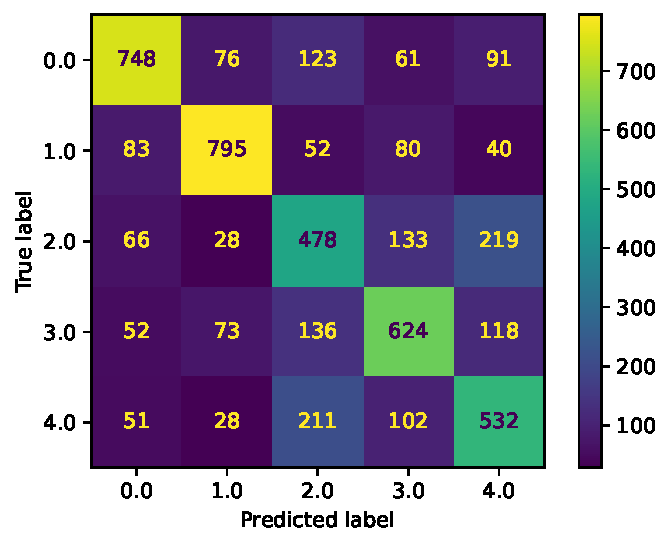
\includegraphics[width=0.44\textwidth]{../Q3/Qc/sk_cmat.pdf} & 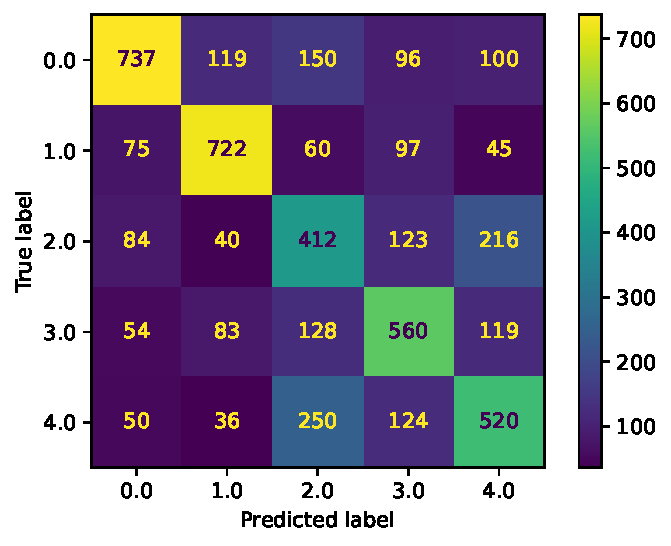
\includegraphics[width=0.44\textwidth]{../Q3/Qc/qp_cmat.pdf} \\
            Scikit & CVXOPT (QP)
        \end{tabular}
    \end{center}

    Classes 2 and 4 are most often misinterpreted as each other. Below, we plot 10 randomly chosen examples which are misclassified by Scikit and CVXOPT, with their {\color{red} predicted} and {\color{green} original} labels respectively

    \begin{center}
        \setlength\tabcolsep{1pt}
        \begin{tabular}{c c c c c c c c c c c}
            &
            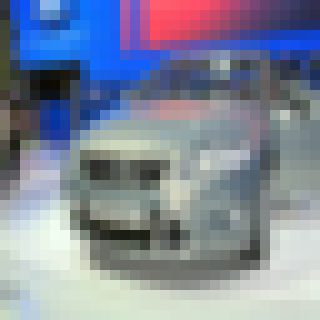
\includegraphics[width=0.08\textwidth]{../Q3/Qc/mc_qp_01_4.png} &
            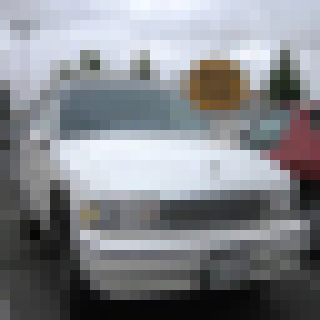
\includegraphics[width=0.08\textwidth]{../Q3/Qc/mc_qp_01_9.png} &
            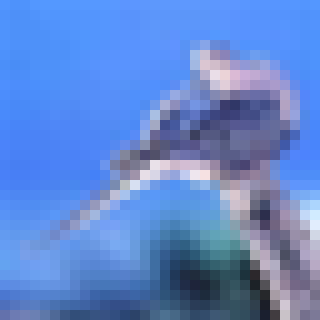
\includegraphics[width=0.08\textwidth]{../Q3/Qc/mc_qp_02_7.png} &
            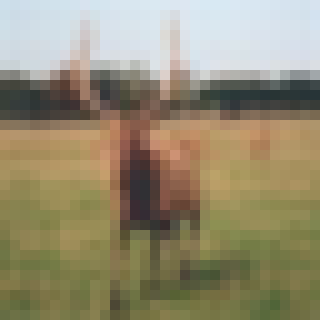
\includegraphics[width=0.08\textwidth]{../Q3/Qc/mc_qp_04_6.png} &
            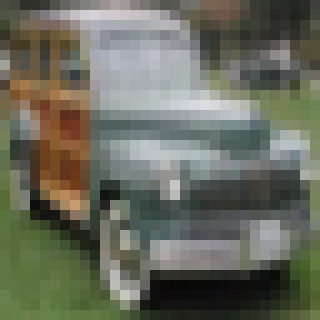
\includegraphics[width=0.08\textwidth]{../Q3/Qc/mc_qp_21_3.png} &
            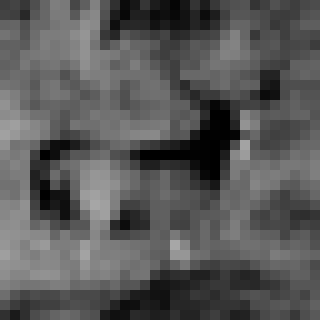
\includegraphics[width=0.08\textwidth]{../Q3/Qc/mc_qp_24_2.png} &
            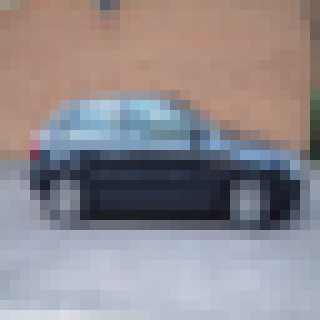
\includegraphics[width=0.08\textwidth]{../Q3/Qc/mc_qp_31_10.png} &
            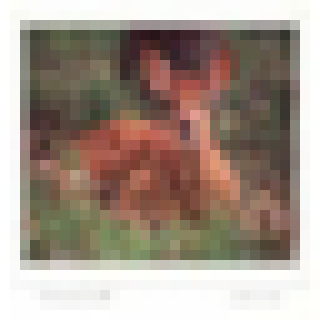
\includegraphics[width=0.08\textwidth]{../Q3/Qc/mc_qp_34_8.png} &
            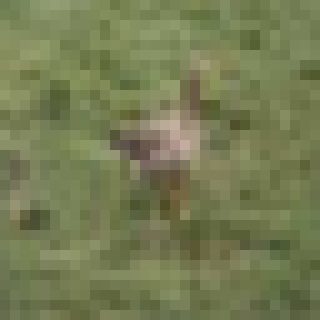
\includegraphics[width=0.08\textwidth]{../Q3/Qc/mc_qp_42_5.png} &
            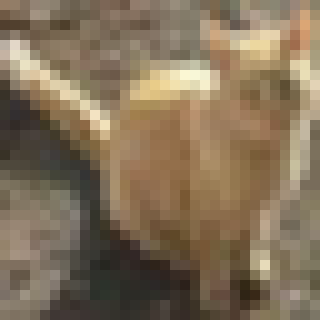
\includegraphics[width=0.08\textwidth]{../Q3/Qc/mc_qp_43_1.png} \\ 
            SK: &
            {\color{red} 0} {\color{green} 1} &
            {\color{red} 0} {\color{green} 1} &
            {\color{red} 0} {\color{green} 2} &
            {\color{red} 0} {\color{green} 4} &
            {\color{red} 2} {\color{green} 1} &
            {\color{red} 2} {\color{green} 4} &
            {\color{red} 3} {\color{green} 1} &
            {\color{red} 3} {\color{green} 4} &
            {\color{red} 4} {\color{green} 2} &
            {\color{red} 4} {\color{green} 3} \\
            &
            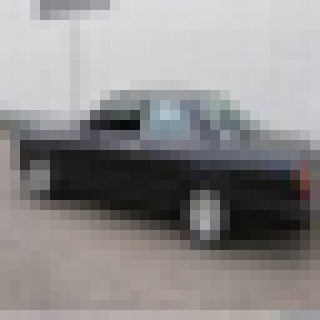
\includegraphics[width=0.08\textwidth]{../Q3/Qc/mc_sk_01_10.png} &
            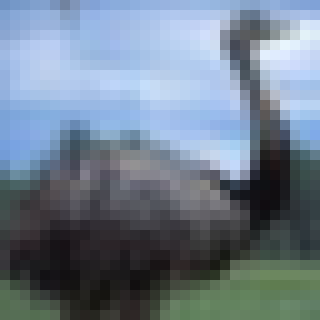
\includegraphics[width=0.08\textwidth]{../Q3/Qc/mc_sk_02_8.png} &
            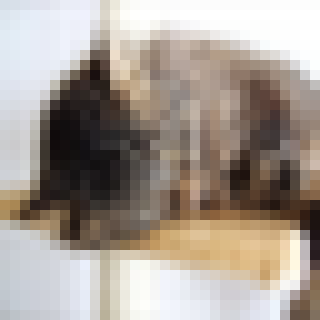
\includegraphics[width=0.08\textwidth]{../Q3/Qc/mc_sk_13_4.png} &
            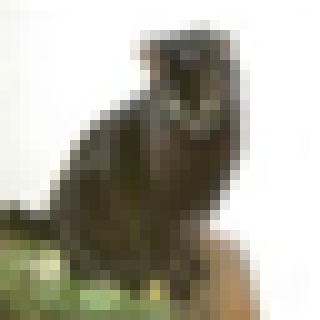
\includegraphics[width=0.08\textwidth]{../Q3/Qc/mc_sk_23_7.png} &
            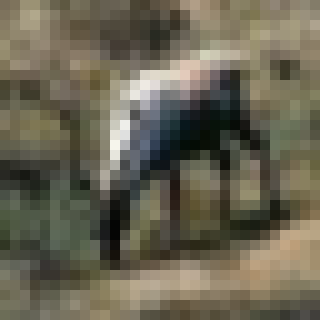
\includegraphics[width=0.08\textwidth]{../Q3/Qc/mc_sk_24_2.png} &
            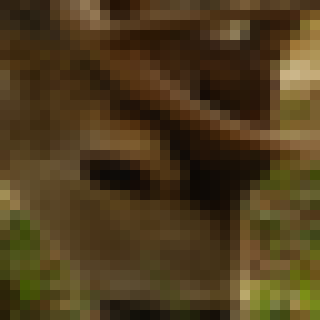
\includegraphics[width=0.08\textwidth]{../Q3/Qc/mc_sk_24_5.png} &
            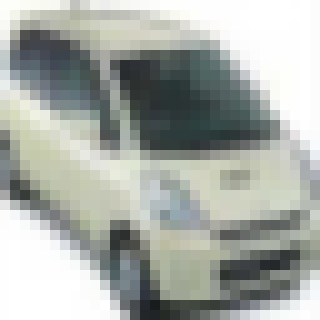
\includegraphics[width=0.08\textwidth]{../Q3/Qc/mc_sk_31_1.png} &
            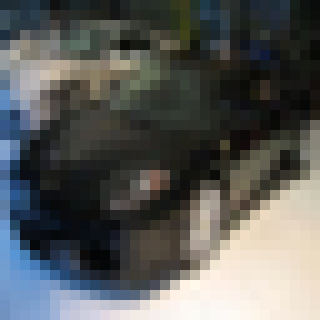
\includegraphics[width=0.08\textwidth]{../Q3/Qc/mc_sk_31_3.png} &
            
\includegraphics[width=0.08\textwidth]{../Q3/Qc/mc_sk_34_9.png} &
            
\includegraphics[width=0.08\textwidth]{../Q3/Qc/mc_sk_42_6.png} \\ 
            QP: &
            {\color{red} 0} {\color{green} 1} &
            {\color{red} 0} {\color{green} 2} &
            {\color{red} 1} {\color{green} 3} &
            {\color{red} 2} {\color{green} 3} &
            {\color{red} 2} {\color{green} 4} &
            {\color{red} 2} {\color{green} 4} &
            {\color{red} 3} {\color{green} 1} &
            {\color{red} 3} {\color{green} 1} &
            {\color{red} 3} {\color{green} 4} &
            {\color{red} 4} {\color{green} 2} \\
        \end{tabular}
    \end{center}

    The classes of the CIFAR-10 dataset are Airplane(0), Automobile(1), Bird(2), Cat(3) and Deer(4). The model(s) misclassify several examples in the bird, cat and deer categories amongst each other, which is to be expected as the backgrounds in which these animals are present is similar. Similarly, Airplanes and Automobiles are most commonly confused with each other rather than with birds, cats or deer because they have similar features (large regions of the same colour, with an urban or blue background).

    \item The plot is given on the following page. We see an increasing trend, where the best accuracy is given by the 'hardest' classifier i.e. for $C = 10$. This value also gives the best test set accuracy. 
        
        The value of C tells the classifier how much we want to avoid misclassifying each example: larger values of C will mean less misclassifications on the training dataset, but this may lead to overfitting. In our case, for small values of C, the model underfits, and chooses a very broad decision boundary, leading to poor cross-validation/test accuracy

        \begin{center}
            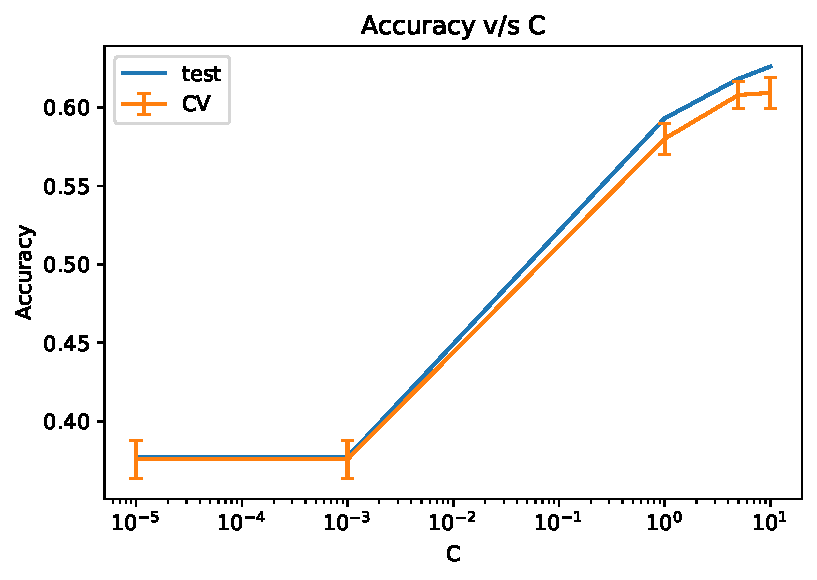
\includegraphics[width=0.7\textwidth]{../Q3/Qd/acc.pdf}
        \end{center}

\end{enumerate}

\end{document}
